\chapter{Meccanica statistica}
I sistemi macroscopici oggetto dello studio della Termodinamica sono tipicamente costituiti da un numero molto elevato $N$ di componenti macroscopiche variamente interagenti dell'ordine del numero di Avogadro $N_A \simeq 6\times 10^{23}$. Microscopicamente, gli stati $\nu$ del sistema sono caratterizzati da un numero enorme, almeno di ordine $N$, di numeri quantici, o quando l'approssimazione classica è applicabile, di coordinate nello spazio delle fasi. Si supponga, per fissare le idee, che i componenti microscopici di un sistema possano essere trattati come particelle classiche puntiformi. In tal caso, uno stato microscopico, ossia un ``microstato'', è caratterizzato da $2\cdot3N = 6N$ coordinate nello spazio delle fasi delle $N$ particelle
\begin{equation}
    \nu_i \longleftrightarrow (\vq_i,\vp_i) = (q^\alpha_i,p_{\alpha,i}) = (q^A,p_A),
\end{equation}
dove $i = 1,\dots,N$, $\alpha=1,2,3$ e quindi $A = (i,\alpha) = 1,\dots,6N$. Se si considera un sistema quantistico di $N$ oscillatori armonici tridimensionali disaccoppiati, o debolmente accoppiati, una base di microstati è caratterizzata tramite i numeri quantici $\vn_i = n_{i,\alpha}$ degli $N$ oscillatori. Uno stato generico quindi è
\begin{equation}
    \ket{\nu(t)} = \sum_{\{\vn_i\}} c(\{\vn_i\},t)\ket{\vn_1,\dots,\vn_N}.
\end{equation}
L'evoluzione di un microstato $\nu(t)$ è determinata dalle equazioni della dinamica classica o quantistica a seconda del contesto. Nel primo caso, se l'hamiltoniana del sistema è $H(q^A,p_A)$, la dinamica è descritta dalle equazioni di Hamilton
\begin{equation}
\label{eq: equazioni di Hamilton}
    \begin{cases}
        \dot{q}^A = \dfrac{\p H}{\p p_A} \\[2ex]
        \dot{p}_A = -\dfrac{\p H}{\p q^A}
    \end{cases},\quad A = 1,\dots,6N.
\end{equation}
Tramite le equazioni \eqref{eq: equazioni di Hamilton} e la conoscenza esatta di $6N$ condizioni iniziali $\{q^A(0),p_A(0)\}$ si può determinare univocamente la traiettoria nello spazio delle fasi che non si autointerseca mai.
\begin{notz}
    In alcune situazioni si può anche usare una notazione vettoriale delle equazioni \eqref{eq: equazioni di Hamilton}
    \begin{equation}
        \begin{cases}
        \dot{\vq}_i = \dfrac{\p H}{\p \vp_i} \\[2ex]
        \dot{\vp}_i = -\dfrac{\p H}{\p \vq_i}
    \end{cases},\quad i = 1,\dots,N.
    \end{equation}
\end{notz}
L'evoluzione dinamica secondo la trattazione classica presenta delle caratteristiche importanti che sono problematiche riguardo all'accordo con la descrizione macroscopica termodinamica. Si mostrano le principali incongruenze.

\paragraph{Reversibilità temporale.} Se il sistema può evolvere lungo una certa traiettoria nello spazio delle fasi, allora anche l'evoluzione inversa è possibile. Quindi, se il sistema evolve dalla situazione iniziale $\{\vq_i(0),\vp_i(0)\}$ allo stato finale $\{\vq_i(t_1),\vp_i(t_1)\}$, allora effettuando l'inversione temporale $t\to t_1 - t'$, si ottiene l'evoluzione inversa dallo stato $\{\vq_i(t'=0),\vp_i(t'=0)\}$ allo stato $\{\vq_i(t'=t_1),\vp_i(t'=t_1)\}$, come mostrato in figura \ref{fig: reversibilità temporale (teo. H)}. Il problema con questa affermazione riguardava la formulazione del teorema H di Boltzmann e il fatto che questo selezionasse una direzione temporale preferenziale, appunto inconsistente con l'invarianza del sistema sotto inversione temporale. Tuttavia, l'incongruenza era solo apparente in quanto l'assunzione su cui si basa è falsa: l'invarianza per inversione temporale non è inconsistente con il teorema H in quanto non è necessario che $\dot{H}$ sia una funzione continua nel tempo. Una spiegazione più chiara di quanto detto verrà esposta in seguito alla derivazione del teorema H.
\begin{figure}[h]
    \centering
    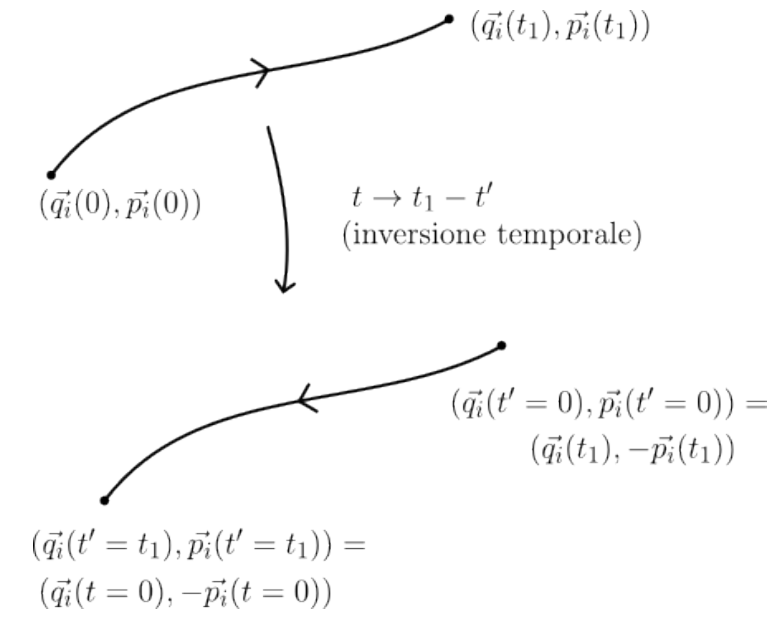
\includegraphics[width=0.5\linewidth]{Immagini/reversibilità temporale (teo. H).png}
    \caption{reversibilità temporale di un sistema.}
    \label{fig: reversibilità temporale (teo. H)}
\end{figure}

\paragraph{Cicli di Poincaré.} Si supponga che il moto del sistema nello spazio delle fasi sia confinato in una regione limitata. Questa richiesta è praticamente sempre verificata in quanto il volume spaziale in cui le componenti di un sistema reale si possono muovere è finito e i momenti non possono tendere all'infinito a causa delle restrizioni imposte dalla Relatività speciale. Si può allora dimostrare che la traiettoria nello spazio delle fasi ripasserà arbitrariamente vicino ad ognuno dei suoi punti, per un generico stato iniziale, dopo un tempo sufficientemente lungo ed escludendo solamente l'insieme degli stati a misura nulla.

\section{Approccio statistico}
Per sistemi microscopici con un numero elevato $N$ di componenti, è di fatto impensabile descriverli classicamente a causa della ridondanza delle $O(N)$ variabili microscopiche. Il comportamento macroscopico all'equilibrio è invece efficacemente descritto tramite poche variabili macroscopiche termodinamiche. Il comportamento del sistema è quindi prevedibile usando i principi della Termodinamica e le particolari equazioni di stato del sistema stesso. In Termodinamica le equazioni di stato dei sistemi sono descritte sperimentalmente. In Meccanica statistica, invece si intende utilizzare la conoscenza della struttura microscopica del sistema per dedurre le equazioni di stato dello stesso. Quando il sistema in equilibrio è caratterizzato da un set di valori delle variabili termodinamiche si dice che si trova in un certo ``macrostato'' di equilibrio. Ad un dato macrostato corrisponde tipicamente un numero enorme di possibili microstati $\nu$. Ad esempio, a fissate $E$, $V$ ed $N$, le particelle di un gas diluito possono essere distribuite, in qualsiasi modo all'interno del volume $V$ e l'energia $E$ può essere distribuita in ogni modo fra di esse. Il sistema nel tempo esplora lo spazio dei possibili microstati, sia che si trovi all'equilibrio, sia che non lo sia per effetto delle interazioni fra le componenti del sistema ed eventualmente del sistema stesso, al più quasi-isolato, con l'ambiente, che ne determina l'evoluzione temporale. Nel farlo, segue una traiettoria $\nu(t)$, passando da un microstato all'altro su una scala temporale $\tau$ tipica della dinamica molecolare, in genere molto breve. In tempi $t \gg \tau$, il sistema visita i possibili microstati con una certa frequenza che all'equilibrio è stazionaria.

Si consideri ora un'osservabile $O$. Una misura affidabile $\tilde{O}$ del suo valore effettuata in un tempo $t \gg \tau$ si può pensare corrisponda alla media di $M$ osservazioni ``istantanee'', ossia svolte in tempo $t \ll \tau$, in modo tale che il sistema si trovi in un definito microstato
\begin{equation}
\label{eq: stima O tramite osservazioni}
    \tilde{O} = \frac{1}{M}\sum_{i = 1}^M \tilde{O}_i.
\end{equation}
Ci si domanda come si potrebbe predire tale risultato a partire dalla conoscenza della struttura microspica. Se fosse possibile determinare in modo esatto l'evoluzione temporale $\nu(t)$ del sistema risolvendo le equazioni di Hamilton, o di Schr\"odinger, e trovando quindi $\{q^A(t),p_A(t)\}$, allora si potrebbe valutare $\tilde{O}$ tramite la media temporale 
\begin{equation}
\label{eq: stima O tramite media temporale}
    \bar{O} = \frac{1}{T}\int_{t_0}^{t_0 + T}dt\,O[\nu(t)].
\end{equation}
Tuttavia, come già detto, questo approccio è impensabile da applicare nel limite di $N\to\infty$ ed in ogni caso risulta inefficiente e ridondante. Invece, si può rimaneggiare l'espressione \eqref{eq: stima O tramite osservazioni} contando il numero di volte $n(\nu)$ in cui appare in essa un certo microstato $\nu$, ottenendo così
\begin{equation}
\label{eq: stima O tramite probabilità (discreta)}
    \tilde{O} = \nsum_{\{\nu\}}\frac{n(\nu)}{M}O(\nu) \simeq \nsum_\nu P(\nu)O(\nu) \equiv \vmedio{O}.
\end{equation}
Infatti, nel limite $M\to\infty$, quindi per un tempo $t$ pari al tempo di misura, si ha $Mt \gg \tau$ e $n(\nu)/M$ è la definizione frequentistica della probabilità $P(\nu)$ che il sistema si trovi nel microstato $\nu$. Nel caso di un sistema classico, dove i microstati corrispondono a punti dello spazio delle fasi, l'espressione discreta \eqref{eq: stima O tramite probabilità (discreta)} passa al continuo diventando
\begin{equation}
\label{eq: stima O tramite probabilità (continua)}
    \tilde{O} \simeq \vmedio{O} = \int dq\,dp\,\rho(\{q^A,p_A\})O(\{q^A,p_A\}),
\end{equation}
dove $\rho(\{q^A,p_A\})\,dq\,dp$ corrisponde alla probabilità che il sistema sia nella porzione di spazio delle fasi compresa tra $[q,q+dq;p,p+dp]$, per cui $\rho(\{q^A,p_A\})$ è una densità di probabilità. 
\begin{notz}
    Per semplicità di notazione, nel seguito si pone $d\mu := dq\,dp$ e $(q,p) \equiv \{q^A,p_A\}$.
\end{notz}
In generale, la condizione perché uno stato sia di equilibrio è che la $\rho(q,p)$ sia stazionaria, mentre in uno stato generico diverso da uno di equilibrio ci si aspetta che $\rho(q,p)$ dipenda esplicitamente dal tempo $t$ risultando in una funzione $\rho(q,p,t)$. Tuttavia, l'evoluzione di $\rho$ è determinata dalle equazioni della Meccanica hamiltoniana microscopica: se si avesse qualche principio che conducesse a determinare $\rho$, almeno all'equilibrio, senza risolvere esplicitamente le equazioni del moto, questo permetterebbe di applicare l'approccio statistico desiderato. 

\subsection{Sottosistemi macroscopici}
Quando si descrive un sistema macroscopico, si può ancora suddividerlo in tanti sottosistemi, ancora macroscopici. Questi sistemi non sono isolati, ma interagiscono in modo continuo con le altre parti del sistema. Dato però che queste parti, piccole rispetto al sistema intero, sono anch'esse corpi macroscopici, è lecito assumere che in intervalli di tempo non troppo lunghi rispetto alla scala temporale $\tau$ della dinamica microscopica, si comportino pressappoco come sistemi isolati. Infatti, sono prevalentemente le particelle che si trovano in prossimità della superficie del sottosistema ad entrare in interazione con le parti circostanti, ma il numero relativo di queste particelle rispetto al numero totale di particelle del sottosistema diminuisce rapidamente quando le sue dimensioni aumentano; inoltre, se il sottosistema è sufficientemente grande, l'energia di interazione con le parti circostanti sarà piccola rispetto alla sua energia interna. Si può quindi affermare che i sottosistemi sono quasi-isolati. In un intervallo di tempo sufficientemente lungo invece, l'effetto dell'interazione tra i sottosistemi, debole che sia, si manifesta in ogni caso, influenzando anche l'interno del sottosistema. Infatti, è proprio questa interazione relativamente debole a permettere l'evoluzione del sottosistema verso l'equilibrio statistico. Questo è il contenuto del teorema di Liouville.
\begin{teo}[di Liouville]
\label{teo: teorema di Liouville}
    Se $\rho(q,p,t)$ è una densità di probabilità che soddisfa l'equazione di continuità, allora 
    \begin{equation}
        \frac{d\rho}{dt} = \frac{\p \rho}{\p t} + \nsum_A\bigg(\frac{\p\rho}{\p q^A}\dot{q}^A + \frac{\p\rho}{\p p_A}\dot{p}_A\bigg) = 0;
    \end{equation}
    che usando le equazioni di Hamilton \eqref{eq: equazioni di Hamilton} risulta equivalente all'equazione di Liouville
    \begin{equation}
    \label{eq: equazione di Liouville}
         \frac{d\rho}{dt} = \frac{\p\rho}{\p t} + \acomm{\rho}{H} = 0
    \end{equation}
\end{teo}
\begin{proof}
    L'equazione di continuità è in generale un'espressione della forma
    \begin{equation}
    \label{eq: equazione di continuità (dim. teo. Liouville)}
        \frac{\p \rho}{\p t} + \nabla\cdot\vj = 0,
    \end{equation}
    dove in questo caso $\rho \equiv \rho(q,p,t)$ è la densità di probabilità in questione e $\vj = (\rho\dot{q}^A,\rho\dot{p}_A)$. Inoltre, $\vj$ è una costante del moto, infatti esplicitamente l'equazione \eqref{eq: equazione di continuità (dim. teo. Liouville)} ha la forma
    \begin{equation}
    \label{eq: espressione esplicita equazione di continuità (dim. teo. Liouville)}
        0 = \frac{\p\rho}{\p t} + \frac{\p(\rho\dot{q}^A)}{\p q^A} + \frac{\p(\rho\dot{p}_A)}{\p p_A} = \frac{\p\rho}{\p t} +  \frac{\p\rho}{\p q^A}\dot{q}^A + \frac{\p\rho}{\p p_A}\dot{p}_A + \rho\bigg(\frac{\p\dot{q}^A}{\p q^A} + \frac{\p\dot{p}_A}{\p q_A}\bigg).
    \end{equation}
    Usando ora le equazioni di Hamilton \eqref{eq: equazioni di Hamilton} si trova che 
    \begin{equation}
        \frac{\p\dot{q}^A}{\p q^A} + \frac{\p\dot{p}_A}{\p q_A} = \frac{\p^2H}{\p q^A\p p_A} -\frac{\p^2H}{\p p_A\p q^A} = 0,
    \end{equation}
    per cui l'ultimo termine della \eqref{eq: espressione esplicita equazione di continuità (dim. teo. Liouville)} si annulla e l'equazione \eqref{eq: equazione di Liouville} segue.
\end{proof}
\begin{obs}
    Si può vedere il teorema di Liouville anche in un altro modo. L'equazione \eqref{eq: equazione di Liouville} corrisponde al fatto che la densità di probabilità nell'intorno di un punto dello spazio delle fasi, vista da un osservatore solidale con l'evoluzione del punto stesso, resta costante. Si può vedere $\rho(q,p,t)$ come un fluido incomprimibile, il cui elemento di volume nello spazio delle fasi viene mantenuto costante durante l'evoluzione dall'hamiltoniana. Infatti, considerando un tratto di evoluzione del sistema dallo stato inziale $(q(0),p(0))$ allo stato finale $(q(t),p(t))$, si ha che al primo ordine, per uno spostamento infinitesimo e usando le equazioni di Hamilton \eqref{eq: equazioni di Hamilton}, si può scrivere
    \begin{equation}
        \begin{cases}
            q(t) \simeq q(0) - \dfrac{\p H}{\p p}\bigg|_{(q(0),p(0))}dt \\
            p(t) \simeq p(0) - \dfrac{\p H}{\p q}\bigg|_{(q(0),p(0))}dt
        \end{cases}.
    \end{equation}
    Quindi, l'elemento di volume si trasforma con lo jacobiano secondo
    \begin{equation}
        dq(0) \wedge dp(0) \to dq(t) \wedge dp(t) = J(t)[dq(0) \wedge dp(0)],
    \end{equation}
    dove per l'appunto 
    \begin{equation}
        \begin{split}
            J(t) &= \det{
            \begin{pmatrix}
                \dfrac{\p q}{\p q(0)} & \dfrac{\p q}{\p p(0)} \\[2ex]
                \dfrac{\p p}{\p q(0)} & \dfrac{\p p}{\p p(0)}
            \end{pmatrix}} \\
            &= \det{
            \begin{pmatrix}
                1 + \dfrac{\p^2 H}{\p q(0)\p p(0)}\,dt & \dfrac{\p^2 H}{\p p(0)^2}\,dt \\[2ex]
                \dfrac{\p^2 H}{\p q(0)^2}\,dt & 1 - \dfrac{\p^2 H}{\p p(0)\p q(0)}\,dt
            \end{pmatrix}} \\
            &\simeq 1 + \bigg(\dfrac{\p^2 H}{\p q(0)\p p(0)} - \dfrac{\p^2 H}{\p q(0)\p p(0)}\bigg)\,dt = 1.
        \end{split}
    \end{equation}
\end{obs}
L'assunzione che l'interazione tra i diversi sottosistemi sia debole permette anche di considerare questi sottosistemi statisticamente indipendenti, per cui lo stato in cui si trova uno dei sottosistemi non influenza in alcun modo sulle probabilità che gli altri sottosistemi si trovino in diversi stati. In termini matematici, questa proprietà si traduce nel fatto che la distribuzione statistica $\rho$ del sottosistema composto da due sottosistemi sia uguale al prodotto delle rispettive funzioni di distribuzioni dei sottosistemi componenti $\rho_1$ e $\rho_2$, ossia $\rho \equiv \rho_{12} = \rho_1\rho_2$. In generale, per un sistema composto da $N$ sottosistemi ognuno caratterizzato da una densità di probabilità $\rho_i$, con $i=1,\dots,N$, si ha che la densità di probabilità complessiva del sistema è
\begin{equation}
\label{eq: ipotesi indipendenza statistica}
    \rho \equiv \rho_{1,\dots,N} = \prod_{i = 1}^N\rho_i.
\end{equation}
A partire da questa assunzione, si consideri nuovamente un'osservabile $O_i$, questa volta relativa al solo sottosistema $i$-esimo. L'indipendenza statistica \eqref{eq: ipotesi indipendenza statistica} implica, considerando un secondo sottosistema $j$, che
\begin{equation}
    \vmedio{O_iO_j} = \vmedio{O_i}\vmedio{O_j};
\end{equation}
infatti è immediato vedere che
\begin{equation}
    \vmedio{O_iO_j} = \int d\mu_i\,d\mu_j\,\rho_{ij}O_iO_j = \int d\mu_i\,\rho_iO_i\int d\mu_j\,\rho_jO_j = \vmedio{O_i}\vmedio{O_j}.
\end{equation}
Si consideri adesso un'osservabile additiva $O$, ossia tale che
\begin{equation}
    \vmedio{O} = \sum_{i = 1}^N\vmedio{O_i} \propto N.
\end{equation}
Dato che l'osservabile $O_i$ varia nel tempo, oscillando intorno al suo valore medio, si introduce la varianza $\sigma^2$, o fluttuazione quadratica media, che caratterizza in media la larghezza dell'intervallo di tale fluttuazione, data da
\begin{equation}
\label{eq: varianza O}
    \begin{split}
        \sigma^2_O &= \vmedio{O^2} - \vmedio{O}^2 \\
        &= \bigvmedio{\bigg(\nsum_iO_i\bigg)^2} - \bigg(\nsum_i\vmedio{O_i}\bigg)^2 \\
        &= \bigvmedio{\nsum_i\nsum_jO_iO_j} - \nsum_i\nsum_j\vmedio{O_i}\vmedio{O_j} \\
        &= \nsum_i(\vmedio{O_i^2} - \vmedio{O_i}^2) + \nsum_{i\neq j}(\vmedio{O_iO_j} - \vmedio{O_i}\vmedio{O_j}) \\
        &= \nsum_i\sigma^2_i,
    \end{split}
\end{equation}
dove nel penultimo passaggio il secondo termine è nulla per l'ipotesi di indipendenza statistica \eqref{eq: ipotesi indipendenza statistica}, mentre li primo coincide proprio con la definizione di varianza per l'osservabile $O_i$ relativa all'$i$-esimo sottosistema. Dal risultato in \eqref{eq: varianza O} si deduce che $\sigma^2_O \propto N$, per cui la fluttuazione è inversamente proporzionale alla radice di $N$
\begin{equation}
    \frac{\sigma_O}{\vmedio{O}} \propto \frac{\sqrt{N}}{N} = \frac{1}{\sqrt{N}}.
\end{equation}
Le fluttuazioni relative delle osservabili additive rispetto ai loro valori medi sono piccolissime nel limite $N\to\infty$. Perciò, per un numero sufficientemente di particelle è lecito assumere che l'osservabile $O$ è praticamente indipendente dal tempo $t$ ed uguale al suo valore medio $\vmedio{O}$. Tale risultato, che si ritrova in effetti dalla trattazione standard della Meccanica Statistica tramite gli ``ensembles'' di Gibbs, giustifica l'approccio statistico stesso in cui valori ``veri'' delle
osservabili vengono identificati con i valori medi estratti tramite una certa distribuzione di probabilità.

Dal teorema di Liouville \eqref{teo: teorema di Liouville}, è immediato dedurre che se si vuole che la densità di probabilità $\rho$ sia stazionaria, necessariamente si deve avere 
\begin{equation}
    \acomm{\rho}{H} = 0.
\end{equation}
Una densità di probabilità $\rho(q,p)$ stazionaria è dunque solo funzione di quantità conservate, ossia di integrali primi del moto. Come già accennato, spiegare come emerga l'equilibrio in cui $\rho$ diventa stazionaria a partire dalla dinamica microscopica che è reversibile rispetto al tempo è problematico e tutt'altro che banale. Tuttavia, dal fatto che $\rho$ dipende unicamente da tali quantità conservate, risulta possibile ridurre notevolmente il numero di integrali primi dai quali $\rho$ può dipendere. A tal fine, si deve tenere conto dell'ipotesi di indipendenza statistica \eqref{eq: ipotesi indipendenza statistica}, dalla quale segue, nel semplice caso di due solo sottosistemi, che
\begin{equation}
    \ln{\rho_{12}} = \ln{\rho_1} + \ln{\rho_2},
\end{equation}
ossia che la quantità $\ln{\rho_{12}}$ è una grandezza additiva. Quindi, si è giunti alla conclusione che il logaritmo della densità di probabilità deve essere non solo un integrale primo, ma anche additivo. Di integrali primi di questo tipo in Meccanica classica ne esistono solo sette; per l'$i$-esimo sottosistema questi sono: l'energia $E_i(q,p)$, le tre componenti del vettore impulso $\vp_i(q,p)$ e le tre componenti del vettore momento angolare $\vL_i(q,p)$. L'unica combinazione additiva di queste grandezze è una combinazione lineare della forma
\begin{equation}
    \ln{\rho_i} = \alpha +\beta E_i(q,p) + \vgamma\cdot\vp_i(q,p) + \vdelta\cdot\vL_i(q,p),
\end{equation}
dove i coefficienti $\alpha$, $\beta$, $\vgamma$ e $\vdelta$ devono essere gli stessi per ogni sottosistema $i$. I valori degli integrali primi additivi determinano completamente le proprietà statistiche del sistema isolato, cioè le distribuzione statistiche di tutti i suoi sottosistemi e quindi i valori medi delle loro grandezze fisiche. L'impulso e il momento angolare di un sistema isolato sono completamente legati al suo moto che sarà di traslazione e rotazione uniforme. Pertanto si può affermare che lo stato statistico di un sistema che compie un dato moto dipende solo dalla sua energia, la quale perciò assume in Meccanica statistica un ruolo del tutto particolare. 

\section{Gerarchia BBGKY}
In Termodinamica emergono comportamenti profondamente diversi da quelli della dinamica microscopica. Infatti, un sistema macroscopico preparato in uno stato generico evolve nel tempo verso lo stato di equilibrio ed uno stato di equilibrio non evolve spontaneamente verso uno stato di non equilibrio. Ci si domanda qundi come questo si possa conciliare con la reversibilità temporale della sottostante dinamica microscopica. 

Uno dei punti chiave per affrontare questo problema è il fatto che le osservabili studiate a livello termodinamico non sono generiche, ma sono legate ad un comportamento collettivo medio delle componenti. In particolare, si considerano le osservabili ``one-body'' $O_1$ definite da
\begin{equation}
\label{eq: definizione osservabili one-body}
    O_1(q,p) := \sum_{i=1}^NO(\vq_i,\vp_i),
\end{equation}
di cui un esempio è l'energia cinetica totale $K$ del sistema
\begin{equation}
    K = \sum_{i=1}^N\frac{|\vp_i|^2}{2m};
\end{equation}
e le osservabili ``two-body'' $O_2$ definite da 
\begin{equation}
\label{eq: definizione osservabili two-body}
    O_2(q,p) := \sum_{i<j=1}^NO(\vq_i,\vp_i;\vp_j,\vp_j),
\end{equation}
di cui un esempio è l'energia potenziale intermolecolare $\Phi$ dipendente dalla distanza relativa
\begin{equation}
    \Phi = \sum_{i<j=1}^N\Phi(|\vq_i - \vq_j|).
\end{equation}
Ora per calcolare il valore medio della variabili ``N-bodies'' non è necessario conoscere la densità di probabilità $\rho$ completa, ma sono sufficienti le densità di probabilità ridotte. 
\begin{notz}
    Per semplicità, nel seguito si indica la distribuzione di probabilità $\rho(\vq_1,\vp_1,\dots,\vq_N,\vp_N;t) \equiv \rho(1,\dots,N;t)$.
\end{notz}
In particolare, per le osservabili one-body si ha
\begin{equation}
    \vmedio{O_1(t)} = \int d\mu_1\cdots d\mu_N\,\sum_{i=1}^NO(\vq_i,\vp_i)\rho(1,\dots,N;t),
\end{equation}
Assumendo che $\rho(1,\dots,N;t)$ sia simmetrica per permutazioni degli argomenti $1,\dots,N$, tutti i contributi sono uguali e pertanto si ottiene
\begin{equation}
    \begin{split}
        \vmedio{O_1(t)} &= N\int d\mu_1\,O(\vq_1,\vp_1)\int d\mu_2\cdots d\mu_N\,\rho(1,\dots,N;t) \\ 
        &= N\int d\mu_1\,O(1)\rho_1(1;t),
    \end{split}
\end{equation}
dove $\rho_1(1;t) \equiv \int d\mu_2\cdots d\mu_N\,\rho(1,\dots,N;t)$ è detta ``densità ridotta di primo ordine''; inoltre, è da notare che si è lasciato libera una particella ed integrato sullo spazio delle fasi su tutte le altre. La normalizzazione di $\rho_1(1;t)$ è
\begin{equation}
    \int d\mu_1\,\rho(1;t) = \int d\mu_1\cdots d\mu_N\rho(1,\dots,N;t) = 1.
\end{equation}
Analogamente, per le osservabili two-body si ha 
\begin{equation}
    \vmedio{O_2(t)} = \int d\mu_1\cdots d\mu_N\,\sum_{i<j=1}^NO(i,j)\rho(1,\dots,N;t).
\end{equation}
Esattamente come prima, per la simmetria rispetto allo scambio degli argomenti di $\rho(1,\dots,N;t)$ tutti i termini danno lo stesso risultato e pertanto si ottiene
\begin{equation}
    \begin{split}
        \vmedio{O_2(t)} &= 
    \begin{pmatrix}
        N \\
        2
    \end{pmatrix}
    \int d\mu_1\,d\mu_2 O(1,2)\int d\mu_3\cdots d\mu_N\rho(1,\dots,N;t) \\
    &= \begin{pmatrix}
        N \\
        2
    \end{pmatrix}
    \int d\mu_1\,d\mu_2 O(1,2)\rho_2(1,2;t),
    \end{split}
\end{equation}
dove $\rho_2(1,2;t) \equiv \int d\mu_3\cdots d\mu_N\rho(1,\dots,N;t)$ è detta densità ridotta di secondo ordine. In un modo analogo, si possono introdurre tutte le densità ridotte di ordine superiore. 

L'insieme delle densità ridotte $\rho_i$ come conseguenza dell'evoluzione di $\rho(1,\dots,N;t)$ dettata dal teorema di Liouville \eqref{teo: teorema di Liouville} soddisfa il sistema gerarchico di equazioni BBGKY che però non è chiuso, nel senso che l'evoluzione di $\rho_1$ dipende da $\rho_2$, quella di $\rho_2$ dipende da $\rho_3$, e così via. Il sistema di equazioni si chiude solo con delle assunzioni aggiuntive. Si consideri il caso particolare dei gas definiti dall'hamiltoniana 
\begin{equation}
\label{eq: hamiltoninana gas}
    H = \nsum_i\frac{|\vp_i|^2}{2m} + \nsum_{i<j}\Phi(|\vq_i - \vq_j|)
\end{equation}
e si assuma che il potenziale sia simmetrico, per cui $\Phi_{ij} = \Phi_{ji}$, e che sia a ``corto raggio'', ossia che si abbia $\Phi_{ij} = 0$ se $|\vq_i - \vq_j| > r_0$, dove $r_0$ è una certa distanza massima di interazione. Dall'hamiltoniana \eqref{eq: hamiltoninana gas} si hanno
\begin{align}
    \nsum_i\frac{\p H}{\p \vp_i} &= \nsum_i\frac{\vp_i}{m}, \\
    \nsum_i\frac{\p H}{\p \vq^i} &= \sum_{k < m} \frac{\p \Phi_{km}}{\p \vq^i} = \sum_{i < m}\frac{\p \Phi_{im}}{\p \vq^i} + \sum_{k < i}\frac{\p \Phi_{ki}}{\p \vq^i} = -\sum_{j\neq i}\vk_{ij},
\end{align}
dove si sono introdotte le forze $\vk_{ij}$ come
\begin{equation}
    \vk_{ij} \equiv -\frac{\p \Phi_{ij}}{\p \vq^i},\quad \vk_{ij} = -\vk_{ji},
\end{equation}
le quali sostituite nell'equazione di Liouville \eqref{eq: equazione di Liouville} restituiscono
\begin{equation}
    \begin{split}
        0 &= \bigg(\frac{\p}{\p t} + \nsum_i\frac{\vp_i}{m}\frac{\p}{\p \vq^i} + \sum_{j\neq i}\vk_{ij}\frac{\p}{\p \vp_i}\bigg)\rho \\
        &= \bigg[\frac{\p}{\p t} + \nsum_i\frac{\vp_i}{m}\frac{\p}{\p \vq^i} + \frac{1}{2}\sum_{j\neq i}\bigg(\vk_{ij}\frac{\p}{\p \vp_i} + \vk_{ji}\frac{\p}{\p \vp_j}\bigg)\bigg] 
        \rho \\
        &= \bigg[\frac{\p}{\p t} + \nsum_i\frac{\vp_i}{m}\frac{\p}{\p \vq^i} + \frac{1}{2}\sum_{j\neq i}\vk_{ij}\cdot\bigg(\frac{\p}{\p \vp_i} - \frac{\p}{\p \vp_j}\bigg)\bigg]\rho,
    \end{split}
\end{equation}
che, introducendo le notazioni
\begin{equation}
    \hatS_i \equiv \frac{\vp_i}{m}\frac{\p}{\p \vq^i},\quad \hatP_{ij} \equiv \vk_{ij}\cdot\bigg(\frac{\p}{\p \vp_i} - \frac{\p}{\p \vp_j}\bigg)
\end{equation}
e definendo l'operatore di Liouville $\hatL_N$ come
\begin{equation}
\label{eq: operatore di Liouville}
    \hatL_N \equiv \nsum_i\hatS_i + \frac{1}{2}\sum_{j\neq i}\hatP_{ij},
\end{equation}
diventa
\begin{equation}
\label{eq: evoluzione temporale densità di probabilità}
    \bigg(\frac{\p}{\p t} + \hatL_N\bigg)\rho = 0.
\end{equation}
Nel seguito, invece delle densità ridotte $\rho_i$ si fa uso delle funzioni di distribuzione $f_s$, che semplicemente hanno una diversa normalizzazione e rappresentano il numero di particelle con determinate coordinate nello spazio delle fasi. In particolare, $f_1(1)$ dipende soltanto dalle variabili ``$1$'' ed è data da\footnote{Più precisamente, è data dal valor medio della somma su tutte le componenti della delta che impone che le coordinate siano proprio certe $\vq^i$ e $\vp_i$ fissate, mentre il fattore $N$ è dovuto al fatto che i tutti i termini della somma contribuiscono allo stesso modo data la simmetria per scambio degli argomenti di $\rho$.}
\begin{equation}
    \begin{split}
        f_1(1) &= \bigvmedio{\sum_{i=1}^N\delta^3(\vq_i - \vq_1)\delta^3(\vp_i - \vp_1)} \\
        &= N\int d\mu_2\cdots d\mu_N\rho(1,\cdots,N) \\
        &= N\rho_1(1).
    \end{split}
\end{equation}
La normalizzazione, come già detto, è diversa da quella della densità ridotta; infatti, se ci si domanda quale sia il numero totale di particelle che si possono trovare in una qualsiasi posizione, la risposta è data dal numero totale di particelle $N$. Pertanto, la normalizzazione è
\begin{equation}
    \int d\mu_1\,f_1(1) = N.
\end{equation}
Analogamente, si può trovare $f_2$ pensandola come la funzione che rappresenta la probabilità congiunta di trovare due particelle aventi specifiche coordinate. Generalizzando il ragionamento, si ha che l'espressione di $f_s \equiv f_s(1,\dots,S)$ è
\begin{equation}
\label{eq: definizione funzioni di struttura}
    \begin{split}
        f_s(1,\dots,S) &= \frac{N!}{(N - S)!}\int d\mu_{s+1}\cdots d\mu_N\rho(1,\dots,S,S+1,\dots,N) \\
        &= \frac{N!}{(N - S)!}\rho_S(1,\dots,S).
    \end{split}
\end{equation}
L'evoluzione temporale di $f_s$ si può determinare usando la \eqref{eq: evoluzione temporale densità di probabilità} ottenendo
\begin{equation}
\label{eq: evoluzione temporale funzioni di distribuzione}
    \begin{split}
        \frac{\p f_s}{\p t} &= \frac{N!}{(N-S)!}\int d\mu_{s+1}\cdots d\mu_N\frac{\p\rho}{\p t} \\
        &= -\frac{N!}{(N-S)!}\int d\mu_{s+1}\,\cdots d\mu_N\hatL_N\rho.
    \end{split}
\end{equation}
Si può scomporre l'operatore di Liouville \eqref{eq: operatore di Liouville} in più termini
\begin{equation}
    \begin{split}
        \hatL_N &= \sum_{i=1}^S\hatS_i + \sum_{j=S+1}^N\hatS_j + \frac{1}{2}\sum_{i\neq j=1}^S\hatP_{ij} + \frac{1}{2}\sum_{i\neq j=S+1}^N\hatP_{ij} + \sum_{i=1}^S\sum_{j=S+1}^N\hatP_{ij} \\
        &= \sum_{i=1}^S\hatS_i + \frac{1}{2}\sum_{i\neq j=1}^S\hatP_{ij} + \sum_{j=S+1}^N\hatS_j + \frac{1}{2}\sum_{i\neq j=S+1}^N\hatP_{ij} + \sum_{i=1}^S\sum_{j=S+1}^N\hatP_{ij} \\
        &= \hatL_S(1,\dots,S) + \hatL_{N-S}(S+1,\dots,N) + \sum_{i=1}^S\sum_{j=S+1}^N\hatP_{ij}.
    \end{split}
\end{equation}
Dunque, l'espressione \eqref{eq: evoluzione temporale funzioni di distribuzione} si può riscrivere come
\begin{equation}
    \begin{split}
        \frac{\p f_s}{\p t} &= -\frac{N!}{(N-S)!}\int d\mu_{s+1}\,\cdots d\mu_N\bigg[\hatL_S(1,\dots,S) \\
        &+ \hatL_{N-S}(S+1,\dots,N) + \sum_{i=1}^S\sum_{j=S+1}^N\hatP_{ij}\bigg]\rho \\
        &= -\frac{N!}{(N-S)!}\int d\mu_{s+1}\,\cdots d\mu_N\bigg[\hatL_S(1,\dots,S) \\
        &+ \sum_{i=1}^S\sum_{j=S+1}^N\hatP_{ij}\bigg]\rho,
    \end{split}
\end{equation}
dove si è considerato che, integrando per parti e assumendo che $\rho$ si annullino ai bordi\footnote{Infatti, $\hatL_{N-S}$ contiene in ogni termine $\p_{\vq^i}$ o $\p_{\vp_i}$ per variabili integrate, moltiplicate per coefficienti indipendenti da tali coordinate, resta così solo il termine di bordo.}, si ha 
\begin{equation}
    \int d\mu_{s+1}\cdots d\mu_N\,\hatL_{N-S}(S+1,\dots,N)\rho(1,\dots,N) = 0.
\end{equation}
Quindi, si ottiene un termine aggiuntivo di evoluzione a sinistra e un temine di collisione a destra
\begin{equation}
    \bigg(\frac{\p}{\p t} + \hatL_S\bigg)f_s(1,\dots,S) = -\frac{N!}{(N-S)!}\int d\mu_{s+1}\cdots d\mu_N\sum_{i=1}^S\sum_{j=S+1}^N\hatP_{ij}\rho.
\end{equation}
Gli $N-S$ termini della sommatoria su $j$ restituiscono lo stesso contributo, per cui si può porre $j=S+1$ e scrivere
\begin{equation}
    \begin{split}
        \bigg(\frac{\p}{\p t} + \hatL_S\bigg)f_s(1,\dots,S;t) &= -\frac{N!(N-S)}{(N-S)!}\sum_{i=1}^S\int d\mu_{s+1}\cdots d\mu_N\hatP_{i,s+1}\rho \\
        &=-\sum_{i=1}^S\int d\mu_{s+1}\,\hatP_{i,s+1}\frac{N!}{[N-(N-S)!]} \\
        &\times\int d\mu_{s+2}\cdots d\mu_N\,\rho,
    \end{split}
\end{equation}
che, ponendo 
\begin{equation}
    f_{s+1}(1,\dots,S+1;t) \equiv \frac{N!}{[N-(S+1)!]} \int d\mu_{s+2}\cdots d\mu_N\rho
\end{equation}
ed esplicitando la forma  di $\hatP_{i,s+1}$, diventa
\begin{multline}
    \bigg(\frac{\p}{\p t} + \hatL_S\bigg)f_s(1,\dots,S;t) = \\
    =-\sum_{i=1}^S\int d\mu_{s+1}\,\vk_{i,s+1}\bigg(\frac{\p}{\p \vp_i} - \frac{\p}{\p \vp_{s+1}}\bigg)f_{s+1}(1,\dots,S+1;t).
\end{multline}
Integrando per parti quest'ultima espressione si può vedere che il termine $\p_{\vp_{s+1}}$ non contribuisce. In definitiva, si ottiene la gerarchia di equazioni BBGKY per le funzioni di distribuzione $f_s$ come
\begin{equation}
\label{eq: gerarchia BBGKY}
    \bigg(\frac{\p}{\p t} + \hatL_S\bigg)f_s(1,\dots,S;t) = \sum_{i=1}^S\int d\mu_{s+1}\,\vk_{s+1,i}\frac{\p}{\p \vp_i}f_{s+1}(1,\dots,S+1;t).
\end{equation}

\section{Equazione del trasporto di Boltzmann}
Dato che per $S = 1$ ed $S = 2$ si hanno
\begin{align}
    \hatL_1 = \frac{\vp_1}{m}\frac{\p}{\p \vp_1},\quad \hatL_2 = \bigg(\frac{\vp_1}{m}\frac{\p}{\p \vp_1} + \frac{\vp_2}{m}\frac{\p}{\p \vp_2}\bigg) + \frac{1}{2}\vk_{12}\bigg(\frac{\p}{\p \vp_1} - \frac{\p}{\p \vp_2}\bigg),
\end{align}
allora la prima equazione della gerarchia BBGKY è
\begin{equation}
\label{eq: I equazione BBGKY}
    \bigg(\frac{\p}{\p t} + \frac{\vp_1}{m}\frac{\p}{\p \vq_1}\bigg)f_1(1) = -\int_{r_0}d\mu_2\,\vk_{12}\frac{\p}{\p \vp_1}f_2(1,2),
\end{equation}
mentre la seconda\footnote{L'estremo inferiore dell'integrale pari a $r_0$ è dovuta all'assunzione che il potenziale di interazione sia a corto raggio.} è
\begin{multline}
\label{eq: II equazione BBGKY}
    \bigg[\frac{\p}{\p t} + \frac{\vp_1}{m}\frac{\p}{\p \vq^1} + \frac{\vp_2}{m}\frac{\p}{\p \vq^2} + \frac{1}{2}\vk_{12}\bigg(\frac{\p}{\p \vp_1} - \frac{\p}{\p \vp_2}\bigg)\bigg]f_2(1,2) = \\
    = -\int_{r_0}d\mu_3\,\bigg(\vk_{13}\frac{\p}{\p \vp_1} - \vk_{23}\frac{\p}{\p \vp_2}\bigg)f_3(1,2,3).
\end{multline}
Nella \eqref{eq: I equazione BBGKY} si ha un termine di scorrimento a sinistra e un termine di collisione a destra, mentre nella \eqref{eq: II equazione BBGKY} si cominciano ad avere termini di collisione anche a sinistra. Per poter rendere la gerarchia BBGKY chiusa si devono fare alcune considerazioni che riguardano in particolare la seconda equazione.

\subsubsection{Ipotesi temporali}
In primo luogo, tutti i termini delle due equazioni sono proporzionali all'inverso di un tempo; in particolare: il termine $\vk\p_{\vp}$ ha le dimensioni di una forza divisa per un impulso che infatti corrisponde all'inverso di un tempo $\tau_c$, che corrisponde al   ``tempo di collisione'', per cui $\vk\p_{\vp} \propto (\tau_c)^{-1}$; il termine $(\vp/m)\p_{\vq}$ ha le dimensioni di una velocità divisa per una posizione e quindi ha ancora le dimensioni di un tempo $\tau_s$, che corrisponde al ``tempo di scorrimento'', ossia il tempo impiegato dalle particelle a percorrere una distanza su cui $f_s$ varia significativamente, per cui  $(\vp/m)\p_{\vq} \propto (\tau_s)^{-1}$.

\subsubsection{Ipotesi del gas diluito}
Tipicamente, si ha che $\tau_c \ll \tau_s$, per cui i termini di collisione sono più rilevanti. Tuttavia, il suo termine di destra è proporzionale alla probabilità di incontrare una terza particella nella zona di interazione. Se si assume che il gas sia diluito, allora la densità di particelle presenti nel volume fondamentale di interazione è molto bassa, quindi l'interazione è trascurabile. Questo termine si può quindi assumere sia proporzionale a $(\tau_x)^{-1}$ tale che 
\begin{equation}
    \frac{1}{\tau_x} \simeq \frac{nr_0^3}{\tau_c},\quad nr_0^3 \ll 1,
\end{equation}
dove $n$ è la densità di particelle e $r_0^3$ è il volume fondamentale di interazione, il cui prodotto è molto piccolo dato che si è supposto che il gas sia diluito. Dunque, questa ipotesi permette di trascurare il secondo membro della \eqref{eq: II equazione BBGKY} eliminando la dipendenza da $f_3$ e rendendo la gerarchia chiusa, inoltre si indica il secondo membro della \eqref{eq: I equazione BBGKY} come $(\p f_1/\p t)_{c}$; quindi si hanno
\begin{equation}
\label{eq: I e II equazioni BBGKY (ipotesi gas diluito)}
    \begin{cases}
        \bigg(\dfrac{\p}{\p t} + \dfrac{\vp_1}{m}\dfrac{\p}{\p \vq_1}\bigg)f_1(1) = \bigg(\dfrac{\p f_1}{\p t}\bigg)_c, \\[2.5ex]
        \bigg[\dfrac{\p}{\p t} + \dfrac{\vp_1}{m}\dfrac{\p}{\p \vq^1} + \dfrac{\vp_2}{m}\dfrac{\p}{\p \vq^2} + \dfrac{1}{2}\vk_{12}\bigg(\dfrac{\p}{\p \vp_1} - \dfrac{\p}{\p \vp_2}\bigg)\bigg]f_2(1,2) = 0.
    \end{cases}
\end{equation}
Dalle precedenti considerazioni temporali, ci si aspetta che $f_2$ evolva molto più rapidamente di $f_1$ e che quindi raggiunga prima una situazione di equilibrio. Inoltre, per via delle interazioni, $f_2$ varia più rapidamente rispetto allo spazio, ovvero $f_1$ misura tempo e spazio su scale più grandi\footnote{In $f_2$, a piccole differenze dell'ordine di $r_0$ possono esserci ampie differenze che $f_1$ non ``vede''.} rispetto a quelle di $f_2$.

\subsubsection{Ipotesi del caos molecolare}
Le correlazioni in $f_2$ sono dovute a collisioni tra le particelle ``$1$'' e ``$2$''. L'ipotesi del caos molecolare consiste nell'assunzione che se la distanza tra le due particelle $|\vq^1 - \vq^2| \ge r_0$, allora non vi sono correlazioni e che quindi si possa scomporre $f_2(1,2;t)$ in due contributi di singola particella, ossia
\begin{equation}
\label{eq: ipotesi caos molecolare}
    f_2(1,2;t) \xrightarrow[|\vq^1 - \vq^2| \ge r_0]{} f_1(1;t)f_1(2;t).
\end{equation}
L'ipotesi del caos molecolare è giustificata a posteriori dal suo successo nel portare all'equazione del trasporto di Boltzmann, permettendo così di predire la forma della distribuzione di Maxwell-Boltzmann per $f_1$ all'equilibrio. Tuttavia, nella prima equazione di \eqref{eq: I e II equazioni BBGKY (ipotesi gas diluito)} compare $f_2$ proprio nella zona di interazione, quindi non è possibile applicare l'ipotesi del caos molecolare per riscrivere l'equazione in funzione solo di $f_1$. Pertanto, per studiare tale zona è conveniente introdurre le coordinate del centro di massa e quelle relative
\begin{equation}
\label{eq: coordinate CM e relative}
    \begin{cases}
        \vR = \dfrac{\vq^1 + \vq^2}{2} \\
        \vr = \vq^2 - \vq^1 
    \end{cases},\quad
    \begin{cases}
        \vP = \vp_1 + \vp_2 \\
        \vp = \dfrac{1}{2}(\vp_2 - \vp_1)
    \end{cases},
\end{equation}
le cui relazioni inverse sono date da
\begin{equation}
\label{eq: coordinate CM e relative (relazioni inverse)}
    \begin{cases}
        \vq^1 = \vR - \dfrac{\vr}{2} \\[2ex]
        \vq^2 = \vR + \dfrac{\vr}{2}
    \end{cases},\quad
    \begin{cases}
        \vp_1 = \dfrac{\vP}{2} - \vp \\[2ex]
        \vp_2 = \dfrac{\vP}{2} + \vp
    \end{cases}.
\end{equation}
Dalle ipotesi di simmetria e di interazione a corto raggio del potenziale $\Phi_{ij}$, si deduce che la forza $\vk_{ij}$ sia solo una funzione della distanza relativa tra le particelle, ossia $\vk_{ij} \equiv \vk_{ij}(\vr)$, inoltre con alcuni passaggi si trova
\begin{equation}
\label{eq: relazione tra coordinate lagrangiane e relative}
    \vp_1\frac{\p}{\p \vq^1} + \vp_2\frac{\p}{\p \vq^2} = \frac{\vP}{2}\frac{\p}{\p \vR} + \frac{\vp}{2}\frac{\p}{\p\vr},
\end{equation}
per cui la seconda equazione di \eqref{eq: I e II equazioni BBGKY (ipotesi gas diluito)} diventa
\begin{equation}
    \bigg[\frac{\p}{\p t} + \frac{\vP}{2m}\frac{\p}{\p \vR} + \frac{\vp}{2m}\frac{\p}{\p \vr} + \frac{\vk(\vr)}{2}\frac{\p}{\p \vp}\bigg]f_2(\vR,\vP,\vr,\vp;t) = 0.
\end{equation}
Si supponga ora per semplicità di porsi nel sistema di riferimento del centro di massa in cui $\vP = 0$, dato che generalizzare al caso generale $\vP \neq 0$ non risulta un problema. Si supponga anche che la distribuzione non dipenda da $\vR$, in quanto non è rilevante la posizione del baricentro. Richiedendo che l'omogeneità sia raggiunta in tempi brevi, si omette l'indicazione della dipendenza da $\vP$ e $\vR$. Quindi, al primo ordine in $dt$ si ha
\begin{equation}
\label{eq: evoluzione temporale f2}
    f_2\bigg(\vp + \vk(\vr)\,dt,\vr + \frac{\vp}{2m}dt;t+dt\bigg) = f_2(\vp,\vr;t),
\end{equation}
la quale codifica l'evoluzione temporale di $f_2$ date le condizioni iniziali. In particolare, determina le traiettorie classiche di una particella di massa ridotta che si muove in un campo di forze $\vk$ centrato in $O$, come mostrato in figura \ref{fig: traiettoria particella in campo forze K}.
\begin{figure}
    \centering
    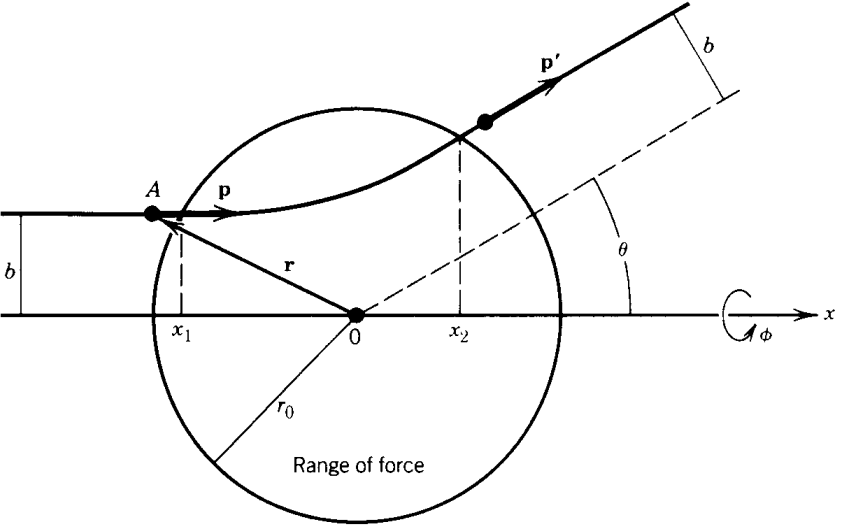
\includegraphics[width=0.6\linewidth]{Immagini/traiettoria particella in campo forze K.png}
    \caption{traiettoria seguita da un particella nel campo di forze $\vk$ centrato in $O$.}
    \label{fig: traiettoria particella in campo forze K}
\end{figure}
Quindi, sempre con riferimento alla figura \ref{fig: traiettoria particella in campo forze K}, si ha un campo di forze agente solo all'interno di un'area finita di raggio $r_0$. Una particella libera con impulso $\vp$ entra in questa area ad una certa distanza $b$, detta ``parametro d'impatto''. All'interno dell'area di interazione, la particella subisce l'azione del campo di forze, viene deflessa ed esce dall'area con un momento $\vp'$, in generale diverso dal momento $\vp$ iniziale, allontanandosi con seguendo una nuova traiettoria. La distanza relativa $\vr$ cambia durante l'interazione, mentre a seconda del valore del parametro d'impatto $b$ variano le coordinate $x_1$ e $x_2$ di uscita. In altre parole, le particelle sono correlate solamente all'interno della zona di interazione, ossia della sfera di raggio $r_0$, invece fuori da essa, la funzione di correlazione coincide con il prodotto di due funzioni di distribuzione di singola particella. Se $f_2$ avesse inizialmente un picco\footnote{Qui ci si riferisce al picco della funzione di distribuzione nello spazio delle fasi.} nel punto $A$, tramite l'equazione \eqref{eq: evoluzione temporale f2} si deduce che il picco si muoverebbe lungo la traiettoria classica rappresentata, definita dalle particolari condizioni iniziali. Invece, all'equilibrio si ha $\p_tf_2 = 0$ e pertanto si ha uno stato stazionario di diffusione nel campo di forze $\vk$ di un fascio di particelle con impulso qualsiasi, a tutti i parametri d'impatto $b$. In altre parole, si ha un flusso stazionario di particelle che seguono la traiettoria classica, a seconda del valore di $b$. Dunque, l'ipotesi del caos molecolare può essere ridefinita tramite le seguenti due affermazioni; all'equilibrio:
\begin{enumerate}
    \item fuori dalla regione di interazione non c'è correlazione e vale l'equazione \eqref{eq: ipotesi caos molecolare};
    \item i valori degli impulsi valutati al bordo della regione di interazione sono correlati, ossia dato l'impulso iniziale $\vp$ e il parametro d'impatto $b$, si può prevedere il valore dell'impulso correlato $\vp'$ a seguito della diffusione.
\end{enumerate}

\subsection{Determinazione di \texorpdfstring{$f_1$}{f1}}
L'obiettivo è adesso quello di determinare la funzione di distribuzione $f_1$. Per farlo, si riparte dalle equazioni \eqref{eq: I e II equazioni BBGKY (ipotesi gas diluito)} supponendo che $f_2$ abbia già raggiunto una situazione di equilibrio, così da ottenere
\begin{equation}
\label{eq: I e II equazioni BBGKY (ipotesi gas diluito + f2 equilibrio)}
    \begin{cases}
        \bigg(\dfrac{\p}{\p t} + \dfrac{\vp_1}{m}\dfrac{\p}{\p \vq_1}\bigg)f_1(1) = \bigg(\dfrac{\p f_1}{\p t}\bigg)_c, \\[2.5ex]
        \bigg[\dfrac{\vp_1}{m}\dfrac{\p}{\p \vq^1} + \dfrac{\vp_2}{m}\dfrac{\p}{\p \vq^2} + \dfrac{1}{2}\vk_{12}\bigg(\dfrac{\p}{\p \vp_1} - \dfrac{\p}{\p \vp_2}\bigg)\bigg]f_2(1,2) = 0.
    \end{cases}
\end{equation}
Riscrivendo la seconda equazione di \eqref{eq: I e II equazioni BBGKY (ipotesi gas diluito + f2 equilibrio)} come
\begin{equation}
\label{eq: processo di interazione 1 e 2}
    \dfrac{1}{2}\vk_{12}\bigg(\dfrac{\p}{\p \vp_1} - \dfrac{\p}{\p \vp_2}\bigg)f_2(1,2) = - \bigg(\frac{\vp_1}{m}\dfrac{\p}{\p \vq^1} + \frac{\vp_2}{m}\dfrac{\p}{\p \vq^2}\bigg) f_2
\end{equation}
e sostituendola nella prima, opportunamente arrangiata, sempre di \eqref{eq: I e II equazioni BBGKY (ipotesi gas diluito + f2 equilibrio)}, si ottiene
\begin{equation}
    \begin{split}
        \bigg(\frac{\p f_1}{\p t}\bigg)_c &= -\int_{r_0}d\mu_2\,\vk_{12}\frac{\p}{\p \vp_1}f_2 \\
        &= -\int_{r_0}d\mu_2\,\vk_{12}\bigg(\frac{\p}{\p \vp_1} - \frac{\p}{\p \vp_2}\bigg)f_2 \\
        &= \frac{2}{m}\int_{r_0}d\mu_2\,\bigg(\vp_1\frac{\p}{\p \vq^1} + \vp_2\frac{\p}{\p \vq^2}\bigg)f_2, 
    \end{split}
\end{equation}
che, a sua volta riscritta in termini delle coordinate del centro di massa e relative \eqref{eq: coordinate CM e relative} e usando la relazione \eqref{eq: relazione tra coordinate lagrangiane e relative}, si ha
\begin{equation}
    \bigg(\frac{\p f_1}{\p t}\bigg)_c = \frac{1}{m}\int_{r_0}d\mu_2\bigg(\vP\frac{\p}{\p \vR} + \vp\frac{\p}{\p \vr}\bigg)f_2.
\end{equation}
Come detto, la funzione $f_1$ varia più lentamente di $f_2$ anche sulle scale spaziali, quindi dal punto di vista di $f_1$, si può considerare che le coordinate prima e dopo l'urto risultino molto simili e pertanto porre $\vq^1\simeq\vq^2$. Inoltre, si può non considerare l'effetto di $\p_{\vR}$ perché nel processo d'urto descritto dalla \eqref{eq: processo di interazione 1 e 2} questo non cambia, essendo la coordinata del baricentro. Dunque, si considera
\begin{equation}
     \bigg(\frac{\p f_1}{\p t}\bigg)_c = \frac{1}{m}\int d^3p_2\int_{r<r_0}d^3r\,\vp\frac{\p f_2}{\p \vr}.
\end{equation}
Dal diagramma in figura \ref{fig: traiettoria particella in campo forze K} si vede che durante la traiettoria vale che
\begin{equation}
    \vp\frac{\p f_2}{\p \vr} = -|\vp|\frac{\p f_2}{\p x},
\end{equation}
inoltre, se si considera un elemento infinitesimo di volume, si ha che questo vale $d^3r = b\,db\,dx\,d\phi$ e quindi si può scrivere
\begin{equation}
    \begin{split}
        \bigg(\frac{\p f_1}{\p t}\bigg)_c &= -\frac{1}{m}\int d^3p_2\,|\vp_2 - \vp_1|\int d\phi\,db\,b\int_{x_1}^{x_2}\frac{\p f_2}{\p x} \\
        &= -\frac{1}{m}\int d^3p_2\,|\vp_2 - \vp_1|\int d\phi\,db\,b[f_2(x_2) - f_2(x_1)],
    \end{split}
\end{equation}
dove gli estremi di integrazione $x_1$ ed $x_2$ sono indipendenti, come si deduce dalla \eqref{eq: processo di interazione 1 e 2}, e dove $f_2(x_1)$ ed $f_2(x_2)$ sono rispettivamente la valutazione di $f_2$ prima e dopo la diffusione. Tuttavia, questi valori di $f_2$ sono valutati sul bordo della regione di interazione. Come detto in precedenza, l'ipotesi del caos molecolare vale unicamente all'interno della regione di interazione: inizialmente si aveva un integrale sulla zona di interazione per cui non si poteva applicare il caos molecolare, ma con le ipotesi fatte si è riusciti a trovare i valori di $f_2$ al bordo di tale regione, dove invece vale il caos molecolare vale. Quindi, è ora possibile rimpiazzare $f_2$ con il prodotto di due funzioni di distribuzione $f_1$ per i due punti
\begin{equation}
    f_2(x_1) \to f_1(\vp_1)f_1(\vp_2),\quad f_2(x_2) \to f_1(\vp_1')f_1(\vp_2'),
\end{equation}
dove $\vp_1$ e $\vp_2$ sono determinati dal processo di diffusione quando gli impulsi iniziali sono $\vp_1$ e $\vp_2$ con un parametro d'impatto $b$. In questa discussione, si è trascurata la dipendenza dalle coordinate $\vq^1$ e $\vq^2$, in quanto si è era considerata l'approssimazione $\vq^1 \simeq \vq^2$. Dunque, si arriva all'espressione
\begin{equation}
\label{eq: espressione f1 in dphi e db}
    \bigg(\frac{\p f_1}{\p t}\bigg)_c = -\frac{1}{m}\int d^3p_2\,|\vp_2 - \vp_1|\int d\phi\,db\,b[f_1(\vp_1')f_1(\vp_2') - f_1(\vp_1)f_1(\vp_2)].
\end{equation}
Il modo in cui compaiono le coordinate è legato alla sezione d'urto differenziale per lo scattering. Si ricorda infatti che, dato un certo flusso di particelle incidenti $I$, per sapere quante particelle vengono diffuse con un certo angolo, si deve calcolare la quantità 
\begin{equation}
    A = I\frac{dG}{d\Omega}d\Omega,
\end{equation}
dove $dG/d\Omega$ è appunto la sezione d'urto differenziale e $A$ è il numero di particelle incidenti diffuse per unità di tempo nell'angolo solido $d\Omega$ intorno alla direzione di $\Omega$.
\begin{figure}[h]
    \centering
    \begin{minipage}[t]{0.55\linewidth}
        \centering
        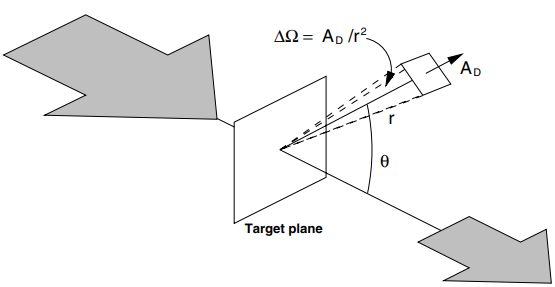
\includegraphics[width=\linewidth]{Immagini/schema scattering.png}
        \caption{schematizzazione della diffusione.}
        \label{fig:schema scattering}
    \end{minipage}
    \hspace{0.8cm}
    \begin{minipage}[t]{0.35\linewidth}
        \centering
        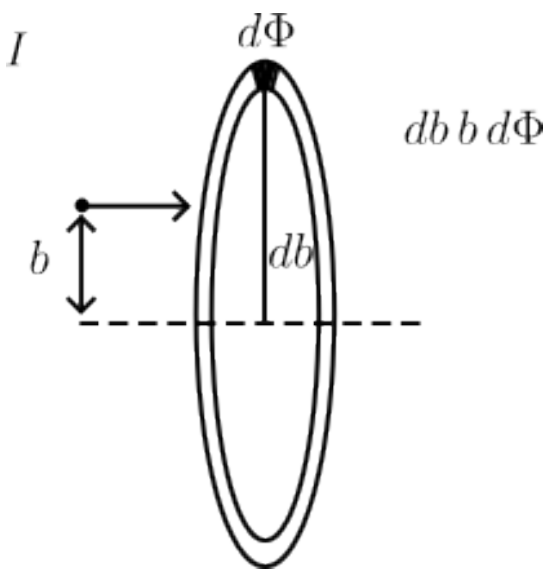
\includegraphics[width=\linewidth]{Immagini/schema per sezione urto.png}
        \caption{analisi per determinare $db\,d\phi$.}
        \label{fig:schema sezione urto}
    \end{minipage}
\end{figure}
Dato che l'angolo di diffusione $\Omega$ è determinato dal parametro d'impatto $b$, sapere qual è il numero di particelle uscenti con un certo angolo $\Omega$ significa conoscere quante sono quelle che entrano con un certo parametro $b$. In altre parole, il numero di particelle diffuse coincide con le particelle entranti in un elemento infinitesimo di superficie perpendicolare al flusso incidente, come mostrato in figura \ref{fig:schema sezione urto}. Quindi, si ha che
\begin{equation}
\label{eq: prodotto db*dphi}
    \cancel{I}\frac{db}{d\Omega}d\Omega = \cancel{I}b\,db\,d\phi\quad\Rightarrow\quad db\,d\phi = \frac{1}{b}\frac{db}{d\Omega}d\Omega.
\end{equation}
Dunque, sostituendo \eqref{eq: prodotto db*dphi} in \eqref{eq: espressione f1 in dphi e db}, si ottiene finalmente l'equazione del trasporto di Boltzmann
\begin{equation}
\label{eq: equazione del trasporto di Boltzmann}
    \bigg(\frac{\p f_1}{\p t}\bigg)_c = -\int d^3p_2\,d\Omega\,|\vv_2 - \vv_1|\frac{db}{d\Omega}\,[f_1(\vp_1')f_1(\vp_2') - f_1(\vp_1)f_1(\vp_2)].
\end{equation}
\begin{notz}
    Per semplicità, dato che nel seguito ci si concentra solo sulla funzione di distribuzione $f_1$, si rinomina $f_1\equiv f$.
\end{notz}
L'equazione del trasporto di Boltzmann fornisce la probabilità che ci siano delle variazioni della funzione di distribuzione di una particella, dovuta alle collisioni con un'altra particella. L'equazione \eqref{eq: equazione del trasporto di Boltzmann} si può reinterpretare come segue
\begin{equation}
\label{eq: equazione del trasporto di Boltzmann in funzione di W}
    \bigg(\frac{\p f}{\p t}\bigg)_c = -\int d^3p_2\,W[(1,2)\to(1',2')][f(2')f(1') - f(2)f(1)],
\end{equation}
dove la funzione $W$ indica la probabilità che avvenga un processo tale per cui lo stato di coppia di particelle $(1,2)$ diventa $(1',2')$, dovuto alla collisione della particella 1 con la particella 2, con $f(1)f(2)$ la probabilità con cui scompare la coppia $(1,2)$, mentre con $f(2')f(1')$ quella con cui compare la coppia $(1',2')$. Dell'equazione \eqref{eq: equazione del trasporto di Boltzmann in funzione di W} si può scrivere l'analogo quantistico
\begin{equation}
\label{eq: equazione del trasporto di Boltzmann quatistica}
    \bigg(\frac{\p f}{\p t}\bigg)_c = -\int d^3p_2\,d^3p_1'\,d^3p_2'\,\delta^4(p_f - p_i)|T_{fi}|^2[f(2')f(1') - f(2)f(1)],
\end{equation}
dove $d^3p_1'\,d^3p_2'$ corrisponde allo spazio delle fasi finale e $|T_{fi}|^2$ è l'elemento di matrice per il processo dallo stato iniziale a quello finale, considerando le possibili interazioni. 

\subsubsection{Distribuzione $f$ all'equilibrio}
Si consideri nuovamente la prima equazione di \eqref{eq: I e II equazioni BBGKY (ipotesi gas diluito)}, dove ora il membro di destra è espresso tramite la \eqref{eq: equazione del trasporto di Boltzmann quatistica}. Si assume che $f \equiv \tilde{f}$ sia in una situazione di equilibrio e che sia omogenea, così da essere indipendente da $\vq^1$, e che sia stazionaria, quindi indipendente da $t$, ovvero $\p_t\tilde{f} = 0$. All'equilibrio continuano ad avvenire fenomeni di scattering tra le particelle, ma questi devono soddisfare la condizione di ``bilancio dettagliato''. Quindi per avere
\begin{equation}
    \bigg(\frac{\p \tilde{f}}{\p t}\bigg)_c = -\int d^3p_2\,d^3p_1'\,d^3p_2'\,\delta^4(p_f - p_i)|T_{fi}|^2[\tilde{f}(2')\tilde{f}(1') - \tilde{f}(2)\tilde{f}(1)] = 0,
\end{equation}
la condizione sufficiente di bilancio dettagliato è ovviamente
\begin{equation}
\label{eq: bilancio dettagliato per f tilde}
    \tilde{f}(2')\tilde{f}(1') = \tilde{f}(2)\tilde{f}(1)\quad\Longrightarrow\quad \p_t\tilde{f} = 0.
\end{equation}
Tuttavia, si può dimostrare che la condizione \eqref{eq: bilancio dettagliato per f tilde} è anche necessaria tramite il teorema H di Boltzmann.

\section{Teorema H}
La quantità $\mathbb{H}$ introdotta da Boltzmann era definita come un funzionale della funzione di distribuzione $f$ in termini della velocità $v$ della particella
\begin{equation}
\label{eq: definizione H}
    \HS = \int d^3v\,f(\vp,t)\log{f(\vp,t)}.
\end{equation}
Se si considerano le proprietà dell'equazione \eqref{eq: definizione H}, è possibile dimostrare, come fece Boltzmann, che essendo $\HS$ limitata inferiormente dal suo valore all'equilibrio, questa non può continuare a decrescere in modo indefinito, ma tende invece al suo valore di equilibrio, mentre contemporaneamente $f$ tende alla distribuzione di Maxwell-Boltzmann. Il teorema H riguarda proprio la dimostrazione dell'andamento non crescente di $\HS$. L'evoluzione temporale di $\HS$ è data da
\begin{equation}
    \frac{d\HS}{dt} = \int d^3v\,\frac{\p f}{\p t}(1 + \log{f}),
\end{equation}
per cui 
\begin{equation}
\label{eq: condizione stazionarietà di f -> stazionarietà di H}
    \frac{\p f}{\p t} = 0 \quad\Rightarrow\quad \frac{d\HS}{dt} = 0
\end{equation}
e la condizione $\dot{\HS} = 0$ è una condizione necessaria affinché $f$ sia stazionaria. Si può dimostrare che la condizione $\dot{H} = 0$ è equivalente a richiedere la relazione di bilancio dettagliato \eqref{eq: bilancio dettagliato per f tilde} quando $f$ soddisfa l'equazione del trasporto di Boltzmann \eqref{eq: equazione del trasporto di Boltzmann}, ossia quando vale l'ipotesi del caos molecolare. Infatti, si considera che 
\begin{equation}
    \begin{split}
        \frac{d\HS}{dt} &= \int d^3v_1\,\frac{\p f(1)}{\p t}(1 + \log{f}) \\
        &= \int\frac{d^3p_1}{m}\bigg(\frac{\p f}{\p t}\bigg)_c[1 + \log{f(1)}] \\
        &= \int\frac{d^3p_1}{m}\int d^3p_2\,d^3p_1'\,d^3p_2'\delta^4(p_f - p_i)|T_{fi}|^2 \\
        &\times[f(1')f(2') - f(1)f(2)][1 + \log{f(1)}].
    \end{split}
\end{equation}
Siccome $|T_{fi}|^2$ è invariante per lo scambio $1 \leftrightarrow 2$ della particella $1$ con la $2$, allora è permesso anche scambiare lo stato iniziale con lo stato finale
\begin{equation}
\label{eq: evoluzione temporale H I}
    \begin{split}
        \frac{d\HS}{dt} &= \frac{1}{2m}\int d^3p_1\,d^3p_2\,d^3p_1'\,d^3p_2'\delta^4(p_f - p_i)|T_{fi}|^2 \\
        &\times[f(1')f(2') - f(1)f(2)][1 + \log{f(1)} + 1 + \log{f(2)}] \\ 
        &= \frac{1}{2m}\int d^3p_1\,d^3p_2\,d^3p_1'\,d^3p_2'\delta^4(p_f - p_i)|T_{fi}|^2 \\
        &\times[f(1')f(2') - f(1)f(2)][2 + \log{f(1)f(2)}].
    \end{split}
\end{equation}
Data l'invarianza di $|T_{fi}|^2$ è anche possibile lo scambio $(1,2) \leftrightarrow (1',2')$ dello stato finale con quello iniziale, ottenendo
\begin{equation}
\label{eq: evoluzione temporale H II}
        \begin{split}
            \frac{d\HS}{dt} &= \frac{1}{2m}\int d^3p_1\,d^3p_2\,d^3p_1'\,d^3p_2'\delta^4(p_f - p_i)|T_{fi}|^2 \\
            &\times[f(1)f(2) - f(1')f(2')][2 + \log{f(1')f(2')}].
        \end{split}
\end{equation}
Le due relazioni trovate \eqref{eq: evoluzione temporale H I} e \eqref{eq: evoluzione temporale H II} sono uguali, pertanto per definire $\dot{H}$ si può considerane una media ottenendo
\begin{equation}
\label{eq: evoluzione temporale H}
    \begin{split}
        \frac{d\HS}{dt} &= \frac{1}{4m}\int d^3p_1\,d^3p_2\,d^3p_1'\,d^3p_2'\delta^4(p_f - p_i)|T_{fi}|^2 \\
        &\times[f(1')f(2') - f(1)f(2)][-\log{f(1')f(2')} + \log{f(1)f(2)}].
    \end{split}
\end{equation}
Per mostrare che l'integrando di \eqref{eq: evoluzione temporale H} non è mai positivo si può considerare la generica funzione di due variabili
\begin{equation}
    h(x,y) = (y - x)(\ln{x} - \ln{y}),\quad x,y > 0,
\end{equation}
dove in questo caso\footnote{In generale, la condizione $x,y > 0$ è relativa al fatto che $x$ ed $y$ sono probabilità.} $y \equiv f(1')f(2')$ e $x \equiv f(1)f(2)$. Quindi, si riscrive $h(x,y)$ come
\begin{equation}
    h(x,y) = y\ln{\bigg(\frac{x}{y}\bigg)}\bigg(1 - \frac{x}{y}\bigg),
\end{equation}
per cui si hanno due casi:
\begin{enumerate}
    \item se il rapporto $x/y \ge 1$, allora $(1 - x/y) \ge 0$ e di conseguenza $h(x,y) \le 0$;
    \item se il rapporto $x/y \le 1$, allora $(1 - x/y) \ge 0$ e di conseguenza $h(x,y) \le 0$.
\end{enumerate}
Dunque, l'equazione \eqref{eq: evoluzione temporale H} coincide con la seguente condizione sul segno di $\HS$ data da $\dot{\HS} \le 0$, particolare il caso di uguaglianza si ha per
\begin{equation}
    \dot{\HS} = 0\quad\Longleftrightarrow\quad \tilde{f}(2')\tilde{f}(1') = \tilde{f}(2)\tilde{f}(1).
\end{equation}
Inoltre, la condizione \eqref{eq: condizione stazionarietà di f -> stazionarietà di H} diventa 
\begin{equation}
    f(1')f(2') - f(1)f(2) = 0 \quad\Longleftarrow\quad \frac{\p f}{\p t} = 0,
\end{equation}
ma si era anche visto dalla \eqref{eq: bilancio dettagliato per f tilde} che 
\begin{equation}
    f(1')f(2') - f(1)f(2) = 0 \quad\Longrightarrow\quad \frac{\p f}{\p t} = 0,
\end{equation}
pertanto le due condizioni sono equivalenti 
\begin{equation}
    f(1')f(2') - f(1)f(2) = 0 \quad\Longleftrightarrow\quad \frac{\p f}{\p t} = 0;
\end{equation}
in particolare, le ipotesi per cui sono equivalenti sono: quella del gas diluito, quella del caos molecolare, quella sull'omogeneità di $f_1$ e il fatto che le variabili $(1,2)$ e $(1',2')$ siano collegate dalla scattering. 

\section{Distribuzione di Maxwell-Boltzmann}
La distribuzione di equilibrio $\tilde{f}(\vp)$ stazionaria deve soddisfare la condizione di bilancio dettagliato \eqref{eq: bilancio dettagliato per f tilde}. 
\begin{notz}
    Per semplicità, nel seguito si indica $\tilde{f} \equiv f$.
\end{notz}
Tale condizione implica che 
\begin{equation}
\label{eq: condizione bilancio dettagliato per f (logaritmica)}
    \log{f(\vp_1')} + \log{f(\vp_2')} = \log{f(\vp_1)} + \log{f(\vp_2)}.
\end{equation}
Si assume ora che lo scattering sia elastico in modo che l'impulso e l'energia cinetica vengano conservati, ossia che
\begin{equation}
    \begin{cases}
        \vp_1 + \vp_2 = \vp_1' + \vp_2' \\
        |\vp_1|^2 + |\vp_2|^2 = |\vp_1'|^2 + |\vp_2'|^2
    \end{cases}.
\end{equation}
La \eqref{eq: condizione bilancio dettagliato per f (logaritmica)} è automaticamente soddisfatta se 
\begin{equation}
    \log{f(\vp)} = a + \vb \cdot \vp - c|\vp|^2,
\end{equation}
dove per ora $a$, $\vb$ e $c$ sono costanti arbitrarie. Se si richiede che la distribuzione di equilibrio corrisponda ad un impulso medio nullo, ovvero che sia invariante per rotazioni, allora deve essere $\vb = 0$, in questo modo la forma generale della funzione di distribuzione risulta essere
\begin{equation}
\label{eq: forma generica distribuzione MB}
    f(\vp) = Ae^{-c|\vp|^2}.
\end{equation}
Si devono adesso imporre alcune condizioni. Prima di tutto, si impone la normalizzazione della funzione $f(\vp)$ come
\begin{equation}
\label{eq: normalizzazione f tilde}
    \int d^3q\,d^3p\,f(\vp) = N,
\end{equation}
inoltre dato che $f(\vp)$ dipende solamente da $|\vp|^2$, allora si può passare in coordinate polari così da avere
\begin{equation}
    \int d^3p\,f(\vp) = 4\pi\int_0^\infty dp\,p^2f(\vp) = \frac{N}{V}.
\end{equation}
Si assume poi nuovamente l'ipotesi del gas diluito, per cui è valida l'equazione di stato termica per i gas monoatomici $E = 3NkT/2$, che adesso si interpreta nel senso che il valor medio dell'energia cinetica per particella debba valere
\begin{equation}
    \bigvmedio{\frac{|\vp|^2}{2m}} = \frac{3}{2}kT,
\end{equation}
da cui segue che
\begin{equation}
\label{eq: ipotesi gas diluito f tilde}
    \int d^3p\,\frac{|\vp|^2}{2m}f(\vp) = \frac{3}{2}\frac{NkT}{V}.
\end{equation}
Passando adesso come prima in coordinate polari, le due condizioni \eqref{eq: normalizzazione f tilde} e \eqref{eq: ipotesi gas diluito f tilde} diventano
\begin{equation}
    \begin{cases}
        4\pi\displaystyle\int_0^\infty dp\,|\vp|^2Ae^{-c|\vp|^2} = \dfrac{N}{V} \\[2ex]
        4\pi\displaystyle\int_0^\infty dp\,\dfrac{|\vp|^4}{2m}Ae^{-c|\vp|^2} = \dfrac{3NkT}{2V}
    \end{cases},
\end{equation}
che, introducendo l'integrale
\begin{equation}
    \int_0^\infty dp\,p^{2k}e^{-cp^2} = \frac{\Gamma(k + 1/2)}{2c^{k + 1/2}} = 
    \begin{cases}
        \dfrac{\Gamma(3/2)}{2c^{3/2}} = \dfrac{\sqrt{\pi}}{4c^{3/2}},\quad k = 1 \\[2ex]
        \dfrac{\Gamma(5/2)}{2c^{5/2}} = \dfrac{3\sqrt{\pi}}{8c^{5/2}},\quad k = 2
    \end{cases},
\end{equation}
diventano
\begin{equation}
\label{eq: normalizzazione f tilde + ipotesi gas diluito f tilde (coord. polari)}
    \begin{cases}
        A\bigg(\dfrac{\pi}{c}\bigg)^{3/2} = \dfrac{N}{V} \\[2ex]
        \dfrac{A}{2mc}\bigg(\dfrac{\pi}{c}\bigg)^{3/2} = \dfrac{NkT}{V}.
    \end{cases}
\end{equation}
Facendo il rapporto delle relazioni \eqref{eq: normalizzazione f tilde + ipotesi gas diluito f tilde (coord. polari)} si trova il valore della costante $c$ come
\begin{equation}
\label{eq: costante c distribuzione MB}
    c = \frac{1}{2mkT},
\end{equation}
il quale sostituito in una delle due condizioni del medesimo sistema restituisce il valore di $A$ come
\begin{equation}
\label{eq: costante A distribuzione MB}
    A = \frac{N}{V(2\pi mkT)^{3/2}}.
\end{equation}
Sostituendo i valori delle due costanti ricavati in \eqref{eq: costante c distribuzione MB} e \eqref{eq: costante A distribuzione MB} nella forma funzionale generica \eqref{eq: forma generica distribuzione MB} si ottiene finalmente la distribuzione di Maxwell-Boltzmann
\begin{equation}
\label{eq: distribuzione MB}
    f(\vp) = \frac{N}{V(2\pi mkT)^{3/2}}\exp{\bigg(-\frac{|\vp|^2}{2mkT}\bigg)}.
\end{equation}

\subsubsection{Osservazioni sul teorema H}
Oltre a determinare la condizione di equilibrio \eqref{eq: bilancio dettagliato per f tilde} individuando così la distribuzione di Maxwell-Boltzmann \eqref{eq: distribuzione MB}, il teorema H di Boltzmann permette anche di affermare che esiste un funzionale $\HS$ della funzione di distribuzione $f$ che per stati diversi da quelli di equilibrio decresce sempre nel tempo. A prima vista, si potrebbe pensare che il funzionale $\HS$ sia in qualche modo proporzionale all'entropia termodinamica $S$ del sistema cambiata di segno. In questo modo, il teorema H sembrerebbe fornire una derivazione dell'irreversibilità macroscopica a partire dalla dinamica microscopica di Liouville. Tuttavia, non è esattamente così, infatti anche se $\HS$ ha un'espressione simile al funzione di entropia di Gibbs, a differenza di $\HS$, l'entropia $S$ non è scritta in termini della funzione di distribuzione della particella singola. Se si prendesse il teorema H come pura conseguenza della dinamica microscopica si andrebbe in contro a dei paradossi, tra cui:
\begin{enumerate}
    \item il ``paradosso dell'irreversibilità'' che riguarda il fatto che il teorema H seleziona una direzione temporale preferenziale che coincide con quella dell'evoluzione irreversibile del sistema, la quale però è incompatibile con la simmetria per inversione temporale della dinamica microscopica;
    \item il ``paradosso della ricorrenza'', legato ai cicli di Poincaré, consiste nel fatto che un sistema preparato in uno stato generico, anche se dovesse raggiungere l'equilibrio, non ci rimarrebbe indefinitamente dato che, su un tempo sufficientemente lungo, il sistema ripassa arbitrariamente vicino allo stato iniziale infinite volte. 
\end{enumerate}
Tuttavia, questi paradossi sono risolti da diverse considerazioni. Inoltre, il teorema H non deriva unicamente dalla dinamica microscopica tramite il teorema di Liouville e le sue conseguenze, ma sfrutta anche l'ipotesi del caos molecolare. In realtà il teorema H afferma che:
\begin{quote}
    ``se ad un istante $t$ vale l'ipotesi del caos molecolare\footnote{L'ipotesi del caos molecolare riguarda $f_2$ non $f_1$, quindi può essere verificata o meno per qualunque $f$.}, allora ad un istante successivo $t' = t + \epsilon$ si ha $\dot{\HS}(t') \le 0$ e la funzione di distribuzione $f(\vp)$ coincide con la distribuzione di Maxwell-Boltzmann.''
\end{quote}
Sfruttando l'invarianza per inversione temporale, si può dedurre che se l'ipotesi del caos molecolare è valida ad un istante $t$, allora si ha
\begin{equation}
    \begin{cases}
        \dfrac{d\HS}{dt} \le 0,\quad t' = t + \epsilon \\[2ex]
        \dfrac{d\HS}{dt} \ge 0,\quad t' = t - \epsilon 
    \end{cases};
\end{equation}
dunque, nell'istante $t$ il funzionale $\HS$ è discontinuo e presenta un picco locale quando vale l'ipotesi del caos molecolare con $f$ che non coincide con la distribuzione di Maxwell-Boltzmann \eqref{eq: distribuzione MB} all'equilibrio, come mostrato in figura \ref{fig: picco locale (teo. H)}.
\begin{figure}[h]
    \centering
    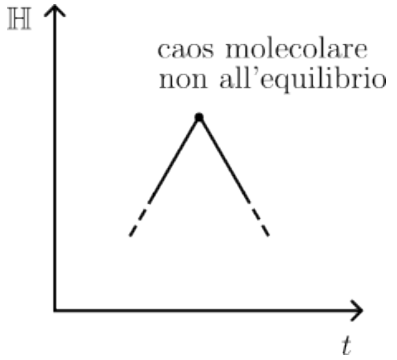
\includegraphics[width=0.35\linewidth]{Immagini/picco locale (teo. H).png}
    \caption{picco locale di $\HS$ fuori dall'equilibrio.}
    \label{fig: picco locale (teo. H)}
\end{figure}

In generale, per un sistema in uno stato diverso da uno di equilibrio non vale l'ipotesi del caos molecolare: gli urti fra le componenti posso crearlo o distruggerlo. L'andamento di $\HS$ riscontrato nelle simulazioni con $N$ abbastanza grande, il quale è in accordo con l'approccio all'equilibrio dei sistemi reali, può essere compreso sulla base delle seguenti, plausibili ma non dimostrate, asserzioni:
\begin{enumerate}
    \item il funzionale $\HS$ è minimo quando la funzione di distribuzione è quella di Maxwell-Boltzmann;
    \item gli urti molecolari hanno un carattere casuale, la sequenza temporale degli stati del gas è scelta casualmente tra i microstati possibili per fissate condizioni macroscopiche;
    \item gli stati di equilibrio sono i più numerosi.
\end{enumerate}
Inoltre, in rifermento al primo grafico in figura \ref{fig: andamento di H}, il comportamento osservato di $\HS$ è il seguente:
\begin{itemize}
    \item se lo stato macroscopico iniziale è prossimo all'equilibrio, vi sono di norma solo piccole fluttuazioni di $\HS$, mentre più $\HS$ si allontana dal valore di equilibrio, più il sistema stesso si è allontana da esso. Tuttavia, questo avviene raramente e il sistema entra ed esce rapidamente da tale stato, con la conseguenza che $\HS$ presenta un picco locale molto pronunciato;
    \item se il sistema viene preparato in uno stato molto fuori equilibrio, siccome tale stato, se occorresse spontaneamente darebbe luogo ad un picco molto pronunciato, è molto probabile un'immediata discesa di $\HS$ che poi ``in media'', ripetendo il ragionamento, continua a scendere verso l'equilibrio.
\end{itemize}
In sostanza, quando il sistema è lontano dall'equilibrio sono più numerose le configurazioni che portano a una diminuzione di $\HS$ rispetto a quelle che la aumentano. Quindi in media $\HS$ decresce, anche se ci sono dei momenti in cui non vale l'ipotesi del caos molecolare. Quindi, il teorema H è una sorta di meccanismo di controllo che impedisce di allontanarsi dall'equilibrio. Questi comportamenti sono stati dimostrati rigorosamente per il modello in cui le particelle sono ``hardspheres'', nel limite dei gas diluiti (teorema di Landford). Si dimostra in tal caso che l'evoluzione di $f$ è guidata dall'equazione di Boltzmann per la stragrande maggioranza degli stati.
\begin{figure}[h]
    \centering
    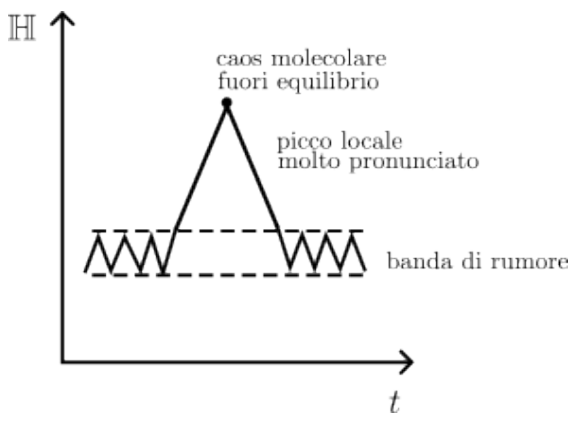
\includegraphics[width=0.45\linewidth]{Immagini/andamento di H (teo. H) 1.png}
    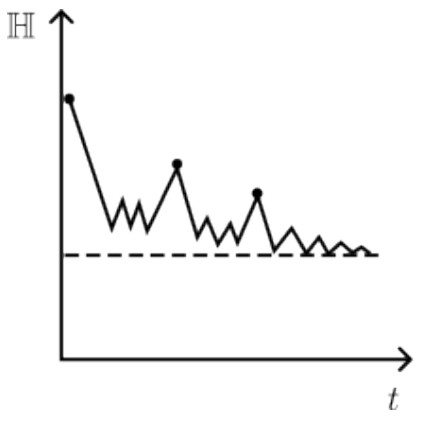
\includegraphics[width=0.35\linewidth]{Immagini/andamento di H (teo. H) 2.png}
    \caption{andamento di $\HS$ per uno stato iniziale: (i) prossimo all'equilibrio; (ii) molto fuori equilibrio.}
    \label{fig: andamento di H}
\end{figure}
